\documentclass[tikz,border=12pt]{standalone}
\usepackage{pgfplots}
\usetikzlibrary{arrows.meta}
\pgfplotsset{compat=1.18}

\definecolor{curveblue}{HTML}{1971C2}
\definecolor{pointpink}{HTML}{C2255C}
\definecolor{linegray}{HTML}{495057}

\begin{document}
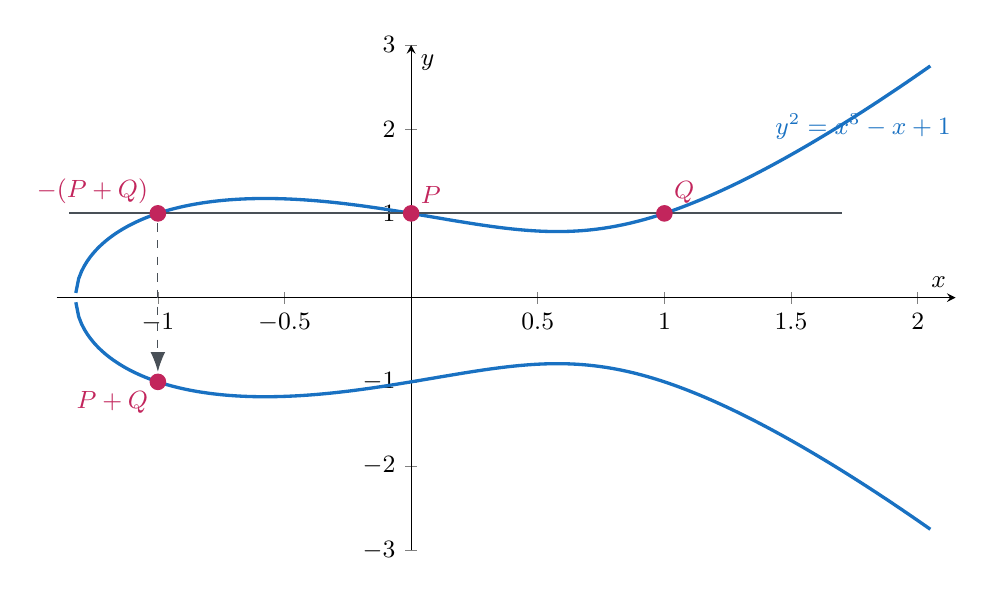
\begin{tikzpicture}
  \begin{axis}[
    width=13cm,
    height=8cm,
    axis lines=middle,
    xmin=-1.4,
    xmax=2.15,
    ymin=-3,
    ymax=3,
    xlabel={$x$},
    ylabel={$y$},
    samples=300,
    tick label style={font=\small},
    label style={font=\small},
    clip=false
  ]
    \addplot[curveblue, very thick, domain=-1.324:2.05] {sqrt(x^3-x+1)};
    \addplot[curveblue, very thick, domain=-1.324:2.05] {-sqrt(x^3-x+1)};
    \addplot[linegray, thick, domain=-1.35:1.7] {1};

    \addplot[only marks, mark=*, mark size=2.8pt, pointpink]
      coordinates {(0,1) (1,1) (-1,1) (-1,-1)};

    \draw[dashed, linegray, -{Latex[length=2.5mm]}]
      (axis cs:-1,0.88) -- (axis cs:-1,-0.88);

    \node[anchor=south west, text=pointpink, font=\small] at (axis cs:0,1) {$P$};
    \node[anchor=south west, text=pointpink, font=\small] at (axis cs:1,1) {$Q$};
    \node[anchor=south east, text=pointpink, font=\small] at (axis cs:-1,1)
      {$-(P+Q)$};
    \node[anchor=north east, text=pointpink, font=\small] at (axis cs:-1,-1)
      {$P+Q$};
    \node[anchor=north west, text=curveblue, font=\small] at (axis cs:1.4,2.3)
      {$y^2=x^3-x+1$};
  \end{axis}
\end{tikzpicture}
\end{document}
